\documentclass{standalonex}
\usepackage{tikz}
\usetikzlibrary{arrows}

\begin{document}
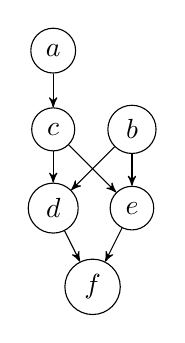
\begin{tikzpicture}[>=stealth']
\node[circle,draw] (a) at (0,3) {$a$};
\node[circle,draw] (c) at (0,2) {$c$};
\node[circle,draw] (b) at (1,2) {$b$};
\node[circle,draw] (d) at (0,1) {$d$};
\node[circle,draw] (e) at (1,1) {$e$};
\node[circle,draw] (f) at (0.5,0) {$f$};
\draw[->] (a) edge (c);
\draw[->] (c) edge (d);
\draw[->] (b) edge (d);
\draw[->] (c) edge (e);
\draw[->] (b) edge (e);
\draw[->] (d) edge (f);
\draw[->] (e) edge (f);
\end{tikzpicture}
\end{document}
